\documentclass{../src/bcthesispart}
\title{Parameter space of the \textsc{dc} language game}
\author{Bas Cornelissen}
\begin{document}

%——————————————————————————————————————————————————————————
\appendixtitle{Parameter space of the \textsc{dc} language game}%
	{Parameter space of the \textsc{dc} language game}%
	{bng-params}{%
	% Abstract
	%---------
	The Bayesian language game has a language strategy parameter $\eta$, a production strategy parameter $\zeta$ and a parameter $\gamma$ for the life expectancy.
	How do those influence the resulting behaviour of the model? 
	This appendix reports an experiment that systematically analysed the behaviour in a larger part of the space.
	}
%——————————————————————————————————————————————————————————

	

The experiment measures three new quantities besides coherence and reflectance
The first concerns the amount of \emph{synonymy} in the language.
If a language assigns all words the same probability, the synonymy is maximal, but if one word takes all probability mass, there is no synonymy. 
Synonymy is the inverse notion of efficiency in the naming games and formally defined as the relative Shannon entropy of the aggregate language,
%-
\begin{align}
	S(t) := 
		\frac{H( \bar{\vect\pi}_t )}%
		{\log_2(N)},
\end{align}
%-
where $H$ is the entropy. $S(t) = 1$ indicates maximal synonymy, $S(t) = 0$ the complete absence of synonymy.
Second, the \emph{discrepancy} between the internal and external language is measured:
%-
\begin{equation}
	D(t) :=
		\textsc{jsd}(\bar{\vect\pi}_t, \vect\psi_t),
\end{equation}
%-
where the aggregate language functioned as a proxy of all internal languages.
Third, we measure the \emph{variability} of the aggregate language as its standard deviation over time,
%-
\begin{align}
	V(t) = \text{std}(\bar{\vect\pi}_0, \dots, \bar{\vect\pi}_t).
\end{align}
%-
If the languages used in the populations were relatively stable throughout the game, the variability should be low.
%%





The experiment simulated 20 runs of the Dirichlet-categorical language game for every combination of the parameters $\eta \in \{1, 2, 5, 50, \infty\}	$, $\zeta \in \{1, 1.5, 2, 5, \infty\}$ and $\gamma \in \{ 1, 10, 50, 10, 100, 1000, \infty \}$.\footnote{%
	%>>>
	To be completely clear: that amounts to 350 million rounds in 3500 independent simulations, using 175 different parameter settings.
	%<<<
	} 
Every run had a duration of 100 000 iterations and all used the same, relatively flat, but nonuniform, prior.
Trial experiments suggested that these parameter values sufficiently illustrate games in different parts of the parameter space.
For example, $\eta>100$ and $\zeta>100$ already yield behaviour comparable to the infinite case and were left out.
The coherence,\footnote{%
	%>>>
	Coherence is not shown, because all simulations appear to have reached coherence.
	This is an artefact of the measure used, which should thus be improved: populations with few observations, as in iterated learning, look perfectly coherent to our measure, because the shared bias fully determines their language.
	%<<<
} reflectance, synonymy, discrepancy, and variability were measured at the end of every game.
Figure \ref{fig:BNG06-parameter-space} shows all the results.
Interpreting the results is tricky, and it helps to keep figure \ref{fig:FIG08-bng-overview} in mind:
The corners of every heat map in figure \ref{fig:BNG06-parameter-space} mark the extreme strategies ($\eta,\zeta\in\{1, \infty\}$), which were also shown in figure \ref{fig:FIG08-bng-overview}.
The life expectancies we considered earlier ($\gamma=1, 10, 100$ and $\infty$) can also be found in figure \ref{fig:FIG08-bng-overview}.
Now, the main conclusion is be that \emph{our earlier findings are largely confirmed by the current experiment.}
For intermediate parameter values, we observe a relatively smooth transition between the extreme cases $\eta,\zeta,\gamma\in\{1,\infty\}$.




%- - - - - - - - 
\begin{SCfigure}
	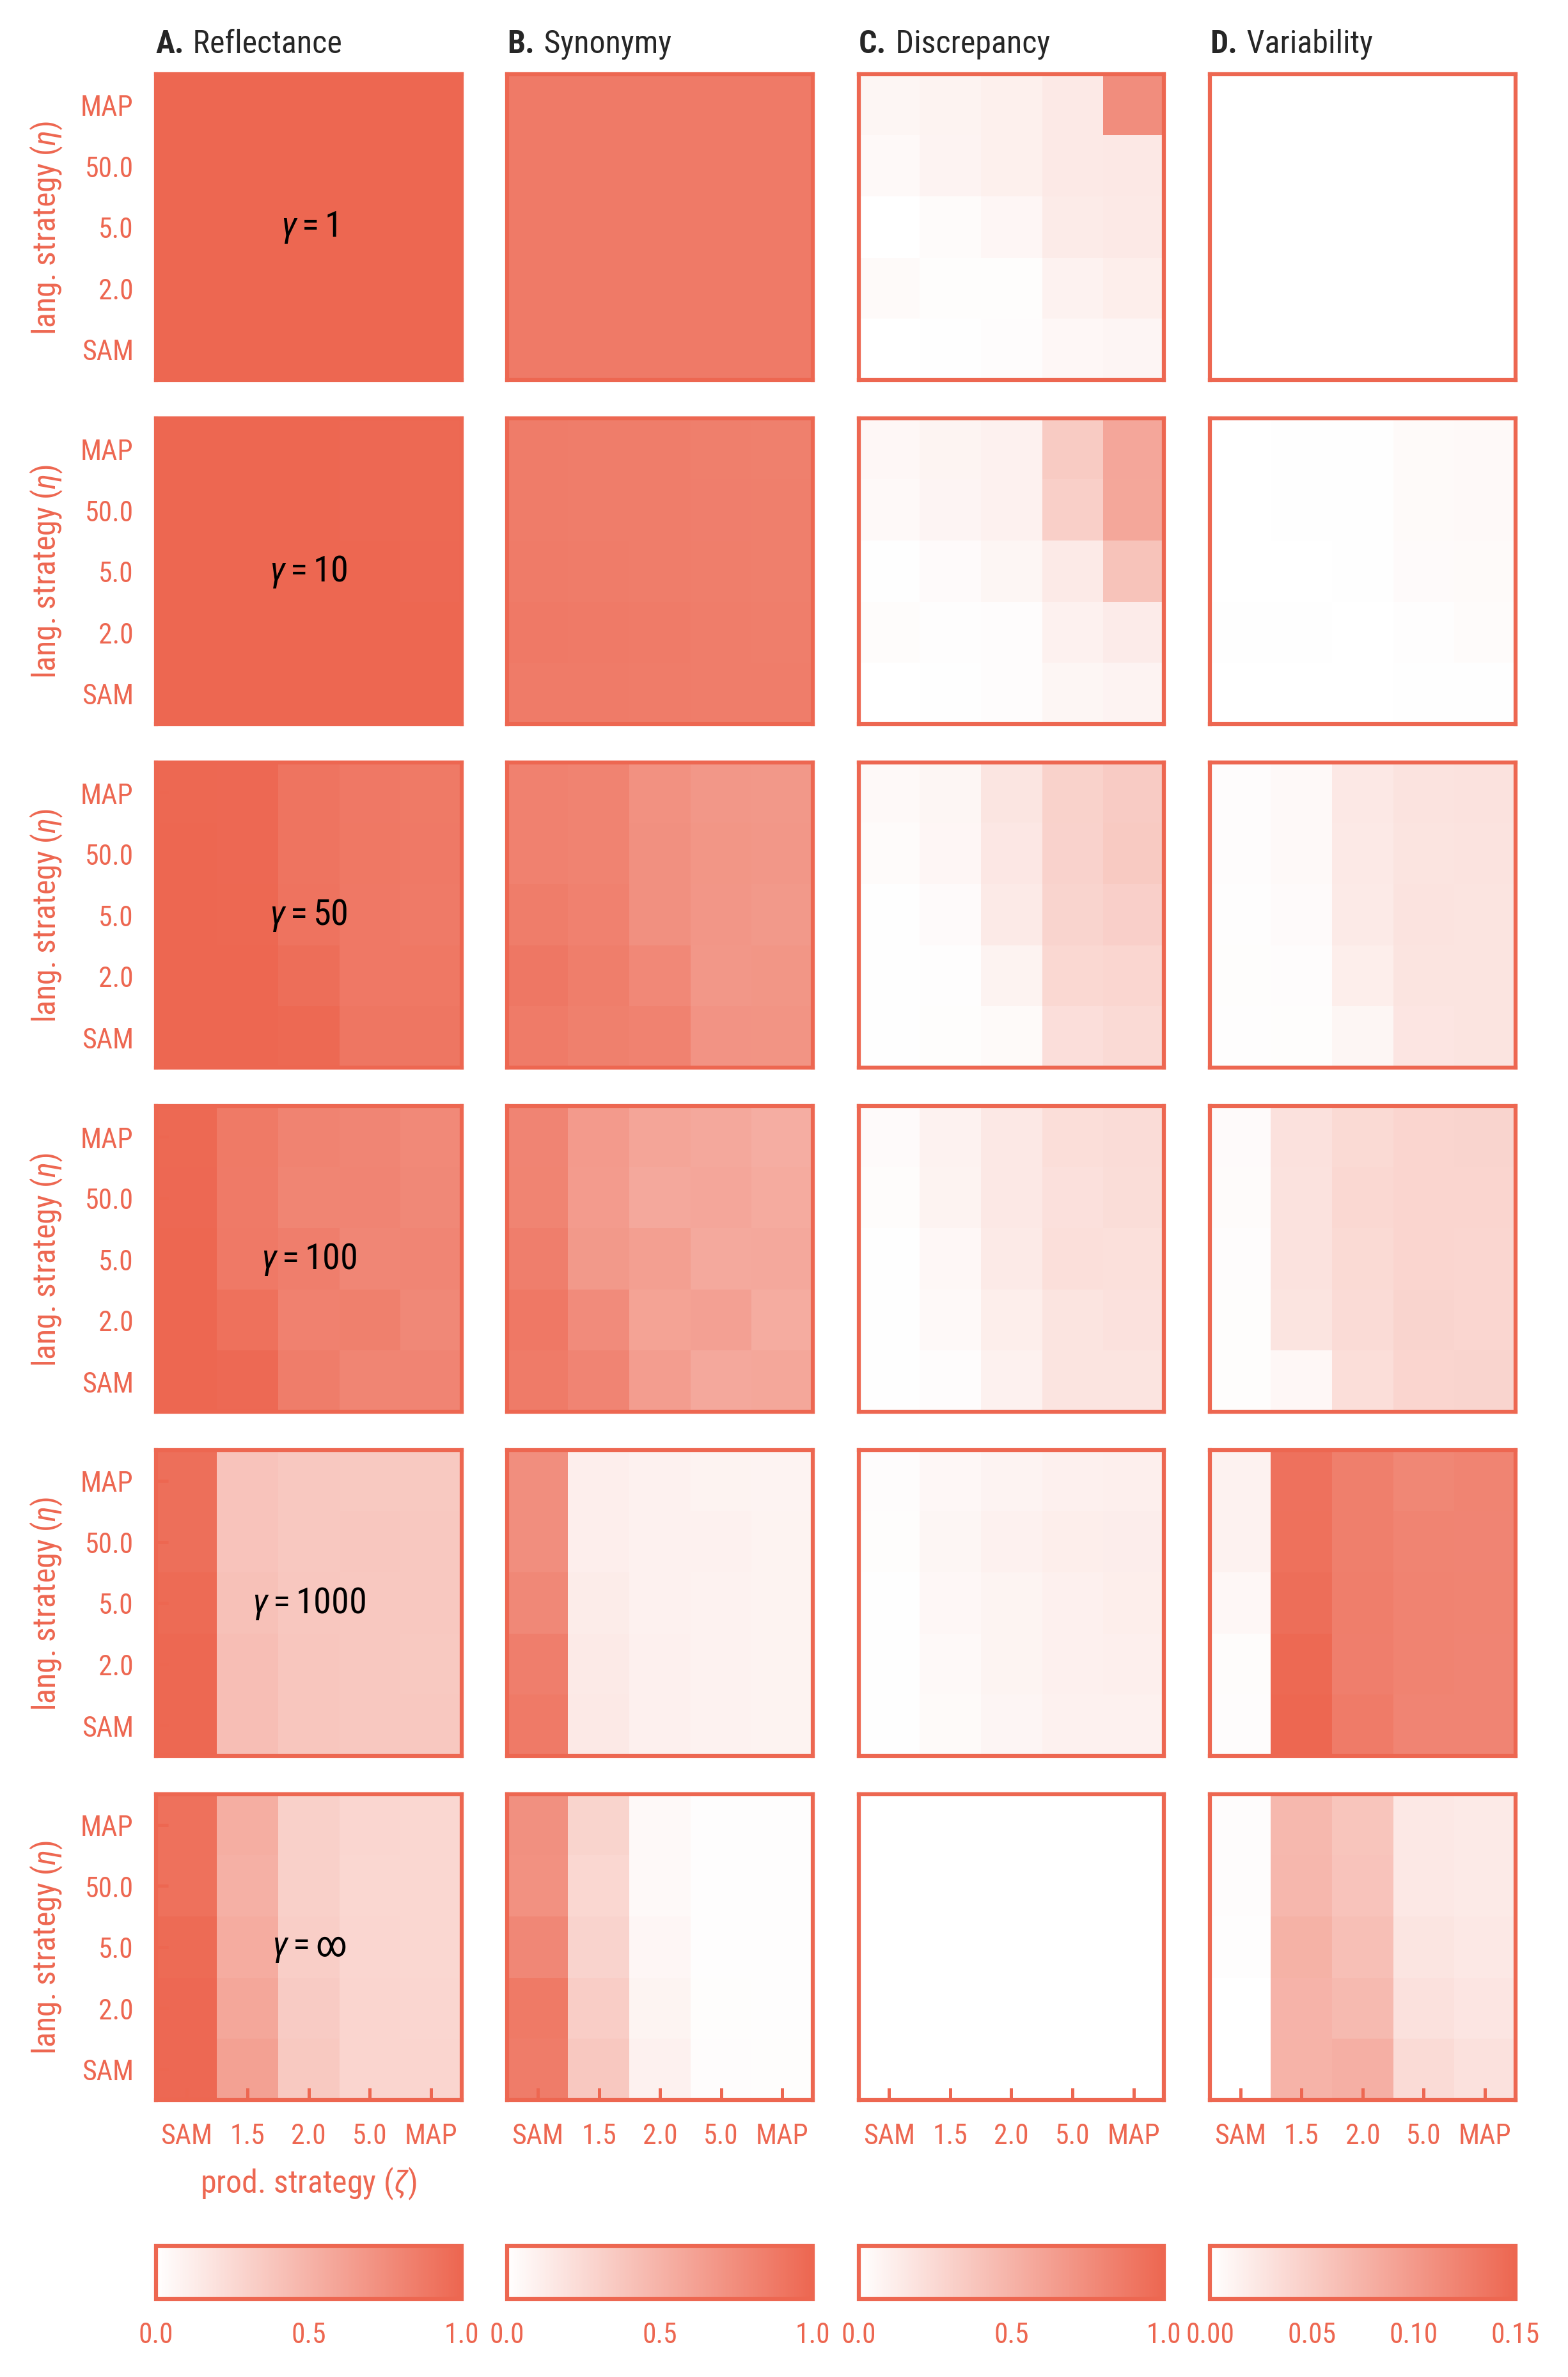
\includegraphics[trim=1.36cm 0 0 \figtopmargin]{BNG06-parameter-space}
	\caption{%
	The behaviour of the Dirichlet-categorical language game across the parameter space $(\gamma,\eta,\zeta)$.
	Rows corresponds to life expectancies ($\gamma$); columns show the coherence, reflectance, synonymy and variability for every strategy $(\eta, \zeta)$.
	See figure \ref{fig:FIG08-bng-overview} for the typical resulting languages in the extreme cases $\gamma,\eta,\zeta \in \{1, \infty\}$.
	%----------
	\figdetails{\figid{bng06}
	Every cell is an average over 20 simulation runs. $K=20$, $N=10$, $b=1$, $\gamma=\infty$, $\beta=30$. 
	Simulations used a deterministic hazard function.}
	\label{fig:BNG06-parameter-space}}
	%todo (optional) highlight extreme cases in plot
\end{SCfigure}
%- - - - - - - - 


We first discuss the last row, which corresponds to a naming game.
The reflectance (column \textsc{a}) is much higher for samplers, and decreases quickly as soon as agents start to maximise their productions slightly (i.e. $\zeta > 1$). 
The synonymy (column \textsc{b}) suggests why: maximising production strategies result in a one-word language, that is, one with no synonymy.
This explains why the reflectance is low for high $\zeta$: the bias allows much more synonymy.
The reflectance and synonymy also suggest that the language strategy ($\eta$) is far less influential than the production strategy ($\zeta$).
The fact that the change in vertical direction is smaller than the change in horizontal direction, and this seems to generalise to other life-spans as well.
Looking at agents with shorter lifespans, we further see that the reflectance and synonymy increase as $\gamma$ approaches 1 (iterated learning).
As before, the reason is that the internal language of an agents with a short life span is nearly completely determined by the bias.
Accordingly, reflectance is high and since the bias is fairly flat, so is synonymy.
But, note that the discrepancy between the external language and the internal  increases sharply for more maximising strategies.
Finally the last column shows an increase in variability with intermediate lifespans. 
This could indicate continuous language change when agents have an intermediate lifespan of around $\gamma=1000$ interactions, but more research is needed before such conclusions are warranted.
%this cannot be concluded yet with any certainty

%Nevertheless, the reflectance and synonymy is largely comparable to the naming-game case ($\gamma=\infty$).
%This suggests that the language is fairly stable, but changes slowly within the constraints set by the bias.




\end{document}
